%% 第八章 系统设计与实现
\chapter{系统设计与实现}

前几章分别解决了检测、跟踪与定位三个算法问题。本章介绍如何将这些算法集成为一套可运行的桌面系统，内容涵盖需求分析、总体架构、算法端实现、显示端实现、通信协议、配置管理、回放与测试框架以及部署运维。

\section{需求分析}

\subsection{功能需求}

根据反无人机监视场景的实际使用流程，本文梳理出以下功能需求：

（1）\textbf{多源视频输入}：支持离线视频文件、USB 摄像头与 TCP 仿真帧流三种输入，便于开发、演示与外场测试；

（2）\textbf{实时目标检测}：对输入视频逐帧检测，输出目标框、置信度与类别；

（3）\textbf{连续目标跟踪}：在目标被短时遮挡时维持航迹，避免标记闪烁；

（4）\textbf{单目定位}：输出目标距离、方位角、俯仰角、速度与三维位置；

（5）\textbf{态势显示}：在卫星地图上标注目标位置、航迹、视野与预测点；

（6）\textbf{光电显示}：显示带检测框的实时画面，叠加准星、刻度与状态；

（7）\textbf{威胁告警}：根据距离与接近速度划分威胁等级，给出视觉与文字告警；

（8）\textbf{数据记录}：逐帧记录检测、跟踪与定位结果，支持离线分析；

（9）\textbf{参数配置}：支持置信度门限、等效尺寸、网络地址、地图锚点等参数的配置与持久化；

（10）\textbf{结果输出}：通过 UDP/JSON 向上级系统输出结构化结果。

\subsection{非功能需求}

除功能需求外，系统还需满足以下非功能需求：

（1）\textbf{实时性}：在 RTX 4060 平台上，端到端处理帧率不低于 20\,fps，界面刷新不低于 10\,Hz；

（2）\textbf{稳定性}：连续运行 2 小时以上不崩溃、不泄漏内存，视频流中断后可自动重连；

（3）\textbf{可移植性}：核心算法与界面解耦，算法端可在无界面环境运行；

（4）\textbf{可测试性}：提供自动化用例与统一日志格式，支持无人值守回归测试；

（5）\textbf{可配置性}：所有关键参数通过配置文件管理，不需要修改代码。

\section{总体架构}

\subsection{双进程结构}

系统采用"算法端—显示端"双进程架构，如图~\ref{fig:sys_arch} 所示。算法端负责视频解码、模型推理、状态机、滤波与记录；显示端负责界面渲染、地图交互与告警。两进程通过 UDP/JSON 通信，也可以运行在同一进程的不同线程中（单机演示模式）。

\begin{figure}[htbp]
\centering
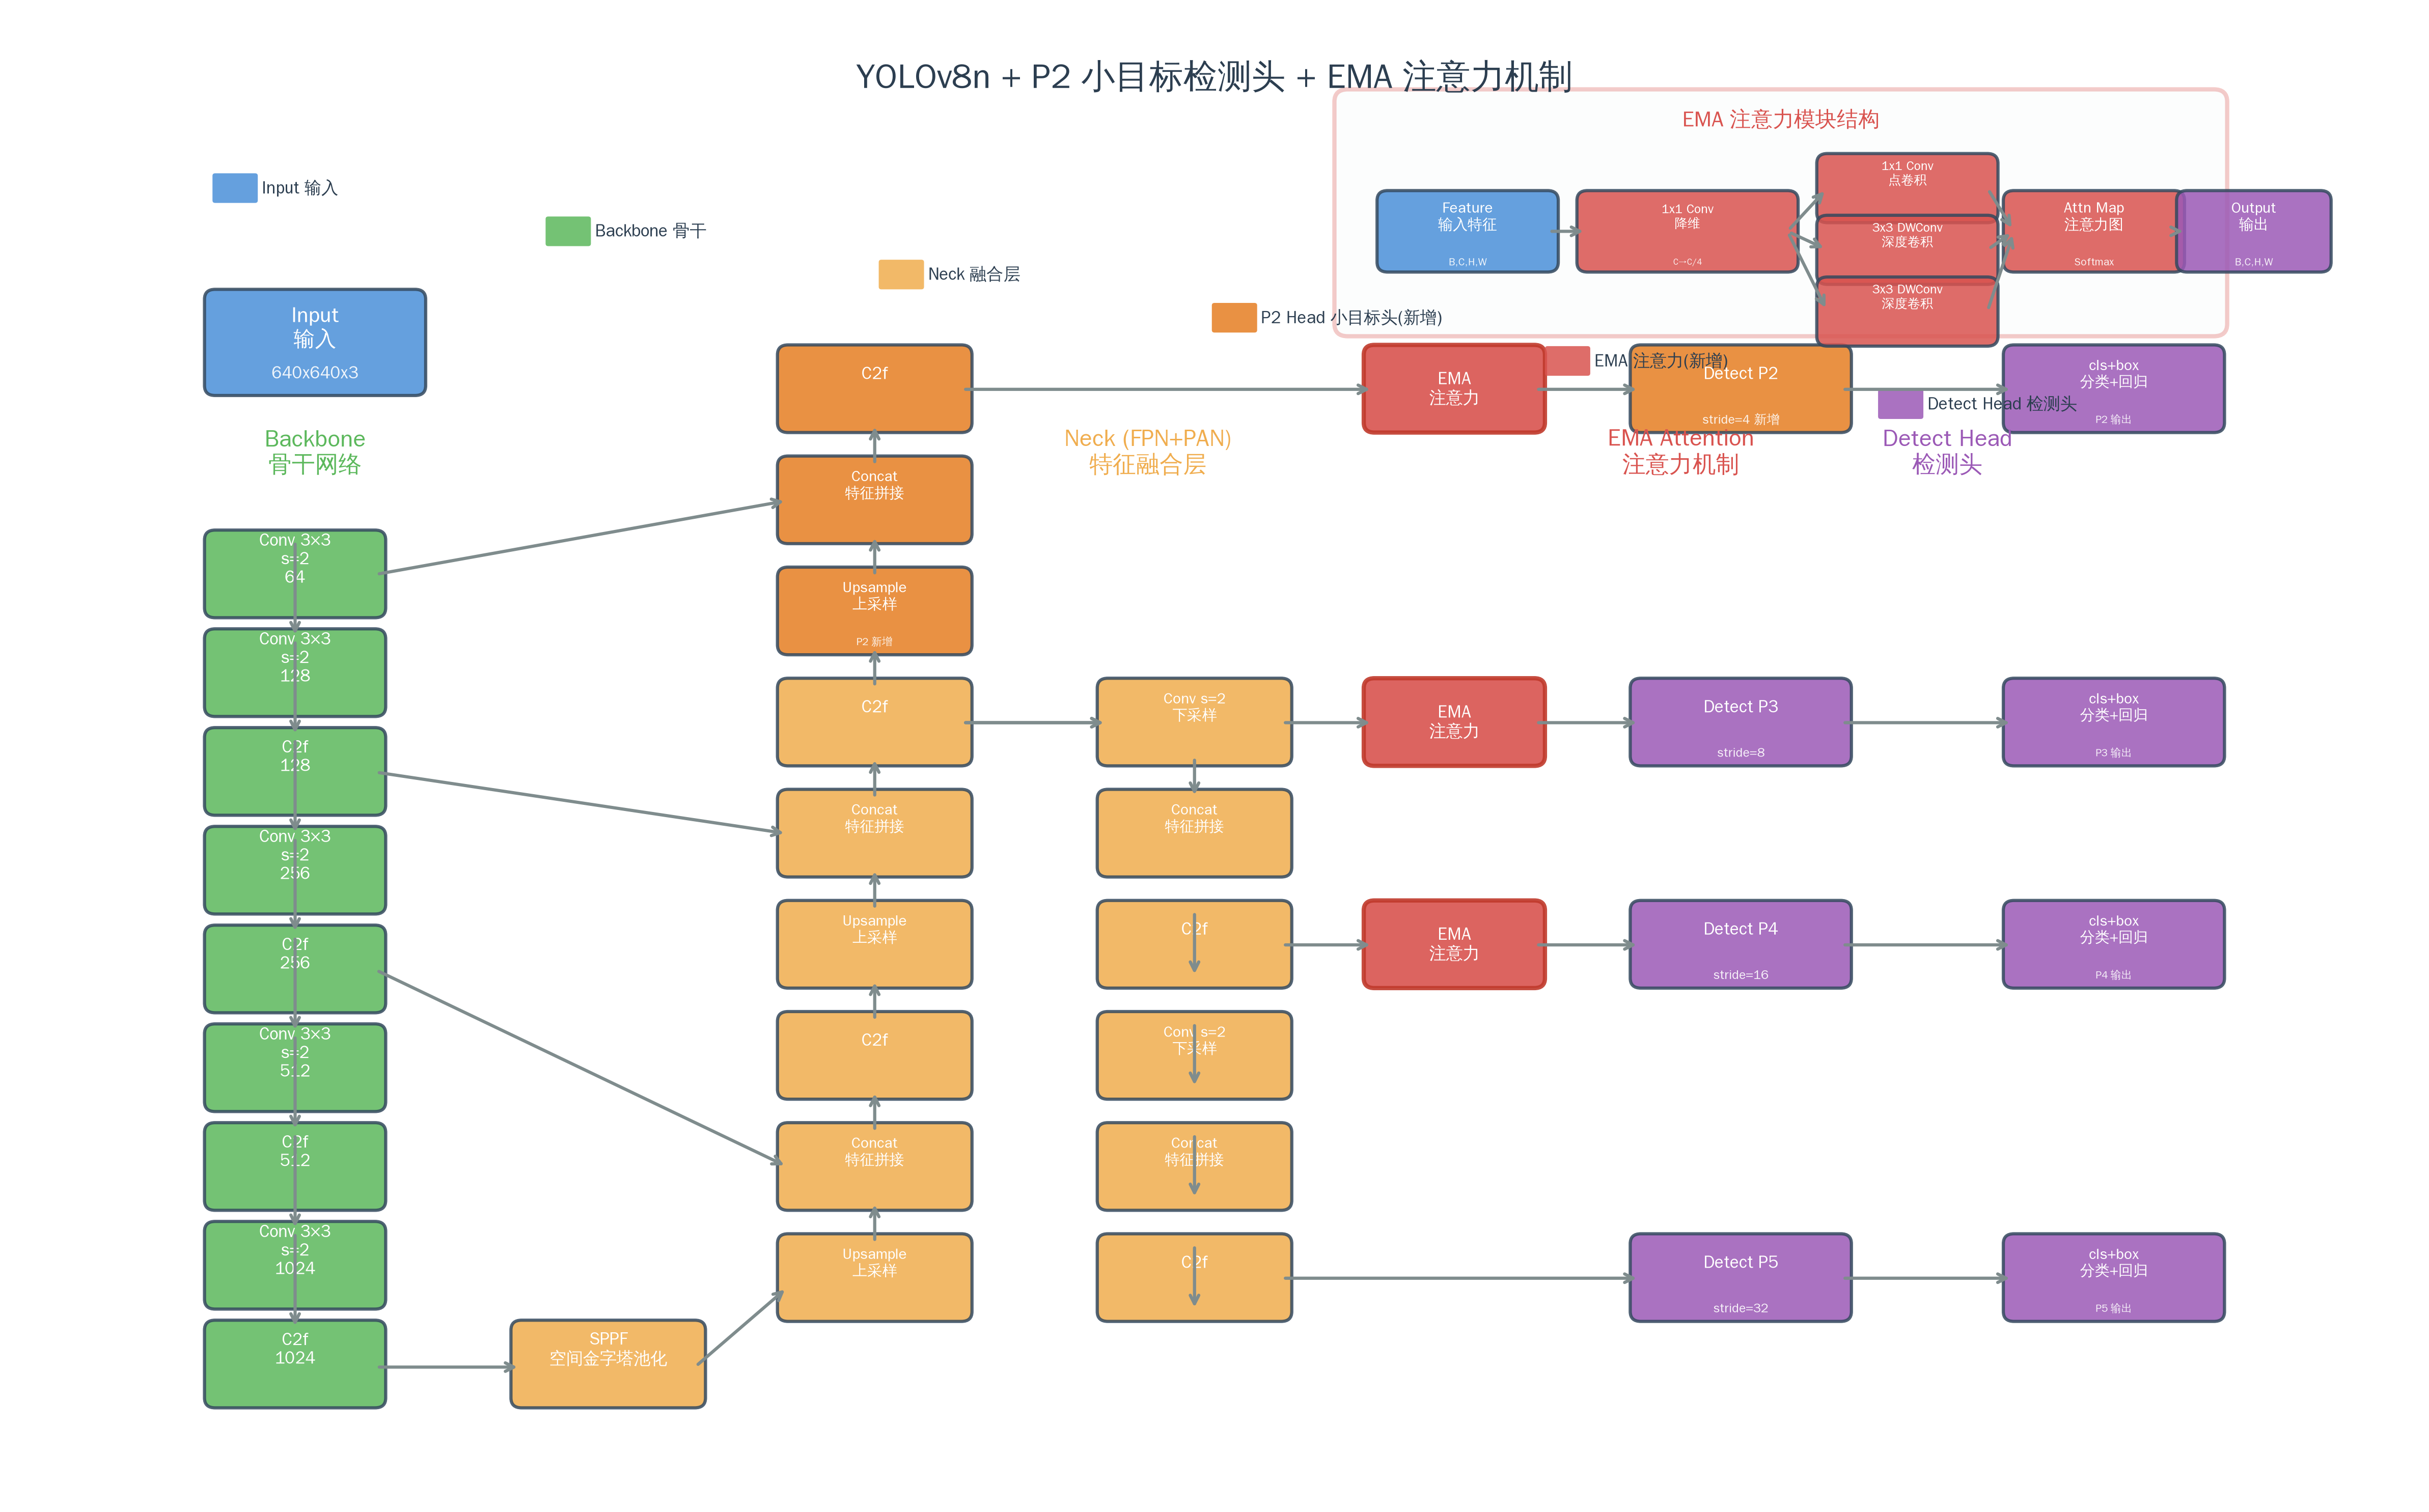
\includegraphics[width=0.95\textwidth]{images/pictures/network_arch.png}
\caption{双进程通信架构}
\label{fig:sys_arch}
\end{figure}

选择双进程架构的理由有三点。第一，\textbf{故障隔离}：检测模型或视频解码可能出现异常，若与界面同进程，异常会导致整个界面崩溃；分离后，算法端异常不会影响界面，显示端可以显示"信号丢失"而不是直接退出。第二，\textbf{部署灵活}：算法端可以部署在带 GPU 的服务器上，显示端部署在操作员的笔记本上，二者通过网络连接。第三，\textbf{调试方便}：算法端可以单独运行并输出 CSV，便于离线分析，不需要启动图形界面。

\subsection{线程模型}

算法端内部采用多线程模型：

（1）\textbf{帧接收线程}：负责 TCP 连接、协议解析与帧解码，将帧放入有界队列；

（2）\textbf{检测线程}：从队列取帧，执行模型推理，将结果放入结果队列；

（3）\textbf{主线程}：执行状态机、滤波、记录与 UDP 输出。

有界队列的作用是背压控制：当检测速度跟不上帧率时，队列满，接收线程会丢弃旧帧而不是无限堆积，保证系统始终处理最新画面。这一设计在长时间运行中尤为重要，避免了内存持续增长。

显示端的主线程负责 Qt 事件循环，另有一个定时器以固定频率从 UDP 接收结果并更新界面。地图更新通过 JavaScript 注入完成，避免频繁重载页面。

\subsection{数据模型}

系统内部统一使用一个结果字典（Python dict）表示单帧输出，主要字段如表~\ref{tab:result_fields} 所示。该字典既用于界面显示，也用于 CSV 记录与 UDP 输出，保证三者的一致性。

\begin{table}[htbp]
\centering
\caption{单帧结果数据字段}
\label{tab:result_fields}
\small
\begin{tabularx}{\textwidth}{llX}
\toprule
\textbf{字段} & \textbf{类型} & \textbf{含义} \\
\midrule
\texttt{frame\_id} & int & 帧序号 \\
\texttt{timestamp} & float & 时间戳（秒） \\
\texttt{det} & bool & 本帧是否检出 \\
\texttt{tracked} & bool & 是否处于跟踪（含 COAST） \\
\texttt{conf} & float & 置信度 \\
\texttt{x1,y1,x2,y2} & int & 检测框像素坐标 \\
\texttt{z\_raw} & float & 单帧原始测距（m） \\
\texttt{z\_akf} & float & 滤波后距离（m） \\
\texttt{z\_pred} & float & 1\,s 预测距离（m） \\
\texttt{azim,elev} & float & 方位角、俯仰角（\textdegree） \\
\texttt{speed} & float & 目标速度（m/s） \\
\texttt{closing} & float & 接近速度（m/s） \\
\texttt{status} & str & SEARCH/LOCKED/COAST \\
\texttt{akf\_cx,akf\_cy} & int & 滤波后中心像素坐标 \\
\texttt{pred\_cx,pred\_cy} & int & 预测中心像素坐标 \\
\bottomrule
\end{tabularx}
\end{table}

\section{算法端实现}

\subsection{视频源抽象}

算法端将三种输入统一为"帧源"接口，提供 \texttt{open}、\texttt{read}、\texttt{close} 三个方法。离线视频源基于 OpenCV 的 \texttt{VideoCapture}；摄像头源同样基于 \texttt{VideoCapture}，但需要处理设备索引与分辨率协商；TCP 帧流源自行实现协议解析，支持断线重连。

TCP 帧流源的读取流程为：

（1）连接服务器地址与端口；

（2）循环读取一行文本头，解析序号、时间戳、宽高与字节数；

（3）按字节数读取 JPEG 数据；

（4）用 \texttt{cv2.imdecode} 解码为 BGR 图像；

（5）若序号跳变，记录丢帧数。

为避免网络抖动导致长时间阻塞，读取设置了超时；超时后关闭连接并重连。

\subsection{检测模块}

检测模块封装 Ultralytics 的 \texttt{YOLO} 类，提供 \texttt{detect(frame)} 方法。实现中做了三项优化：

（1）\textbf{固定输入尺寸}：统一缩放到 640$\times$640，避免动态尺寸导致的重复编译；

（2）\textbf{关闭冗余输出}：设置 \texttt{verbose=False}，减少日志开销；

（3）\textbf{半精度推理}：在 GPU 上使用 FP16，速度提升约 30\%，精度损失可忽略。

检测结果经过非极大值抑制（NMS）后，按置信度降序返回。算法端只保留前 20 个候选框，避免极端场景下的后处理开销。

\subsection{状态机与滤波}

状态机的实现与第五章的伪代码一致，核心是一个 \texttt{update(detections, dt)} 方法。滤波器的实现使用 NumPy 完成矩阵运算，包含预测、更新、自适应噪声估计与数值保护。

实现中特别注意了以下三点：

（1）\textbf{时间步长}：使用实际时间戳差值而非固定 1/30\,s，以兼容不同帧率；

（2）\textbf{数值稳定}：协方差矩阵在每次更新后做对称化处理，避免浮点误差累积导致非正定；

（3）\textbf{状态重置}：目标丢失时清空滤波器与轨迹缓存，避免旧状态污染新目标。

\subsection{数据记录}

算法端在每帧处理完成后，将结果字典追加写入 CSV。表头在文件创建时写入，后续逐行追加。为避免磁盘 I/O 阻塞处理线程，记录采用缓冲写入，每 50 帧刷新一次；程序退出时执行 \texttt{close}，保证数据完整。

CSV 文件按运行时间命名，包含运行参数（模型、门限、尺寸、输入源）的副本，便于后续复现。本文的所有实验数据均来自这些 CSV，分析脚本直接读取 CSV 生成表格与图表。

\subsection{结果输出}

算法端通过 UDP 向显示端发送 JSON 报文，频率与处理帧率一致。报文包含表~\ref{tab:result_fields} 中的主要字段，以及相机位置、时间戳与状态机内部计数。显示端按 \texttt{frame\_id} 去重，只渲染最新报文。

为降低带宽，报文采用紧凑 JSON（无空格），单帧约 300 字节；在 30\,fps 下带宽约 9\,KB/s，对局域网几乎没有压力。

\section{显示端实现}

\subsection{界面布局}

显示端采用三页签布局：目标态势页、检测回放页、参数设置页。目标态势页是主界面，如图~\ref{fig:dashboard_satellite} 所示，分为五个区域：

（1）\textbf{顶部状态栏}：显示系统名称、运行状态、时间与告警等级；

（2）\textbf{左侧信息栏}：目标卡片（类型、距离、置信度、威胁等级）、跟踪状态灯、链路状态；

（3）\textbf{中央地图}：卫星影像底图，标注目标位置、航迹、视野扇形与距离环；

（4）\textbf{右侧仪表}：距离卡、方位罗盘、行动控制按钮；

（5）\textbf{底部数据条}：距离、方位、俯仰、速度、置信度、状态、帧号等 8 项实时数据。

\begin{figure}[htbp]
\centering
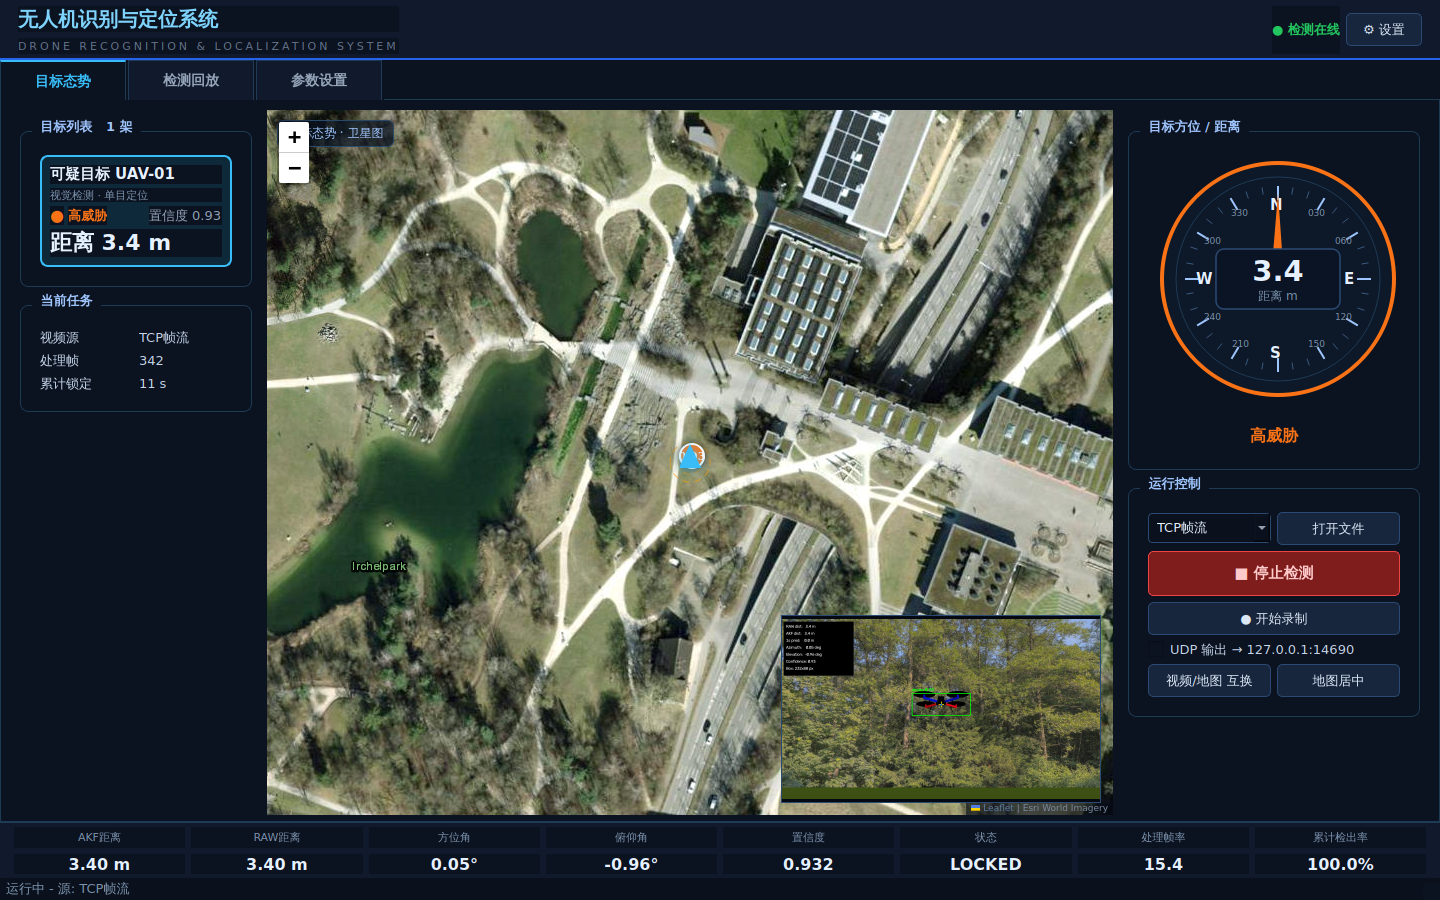
\includegraphics[width=0.98\textwidth]{images/pictures/dashboard_satellite.png}
\caption{目标态势页（卫星地图模式）}
\label{fig:dashboard_satellite}
\end{figure}

\subsection{地图实现}

地图使用 QtWebEngine 嵌入本地 HTML 页面，页面加载 Leaflet 库与 Esri 卫星瓦片。Python 端通过 \texttt{runJavaScript} 向页面推送数据，页面端更新标记位置、折线顶点与圆环半径。

坐标转换是地图实现的关键。算法端输出的目标是相机坐标系下的位置，显示端需要将其转换为经纬度。本文采用局部切平面近似：

\begin{equation}
\phi = \phi_0 + \frac{x_{north}}{R_e},\qquad
\lambda = \lambda_0 + \frac{x_{east}}{R_e\cos\phi_0},
\label{eq:geo}
\end{equation}

其中 $(\phi_0,\lambda_0)$ 为地图锚点（默认取相机机位），$R_e$ 为地球半径，$x_{north},x_{east}$ 为以相机为原点的北向、东向位移。在几百米范围内，该近似的误差小于 0.1\,m，满足监视需求。

地图上叠加了以下元素：

（1）\textbf{观测站标记}：相机位置，随编队移动；

（2）\textbf{目标标记}：实心圆表示 LOCKED，虚线空心圆表示 COAST；

（3）\textbf{预测点}：青色菱形，用虚线与目标标记连接，表示 1\,s 后的预测位置；

（4）\textbf{视野扇形}：以相机为顶点、沿视轴方向的扇形，表示相机覆盖范围；

（5）\textbf{距离同心环}：以相机为圆心，标注 50\,m、100\,m 等距离；

（6）\textbf{航迹折线}：目标历史位置的连线，渐变透明度表示时间新旧。

\subsection{光电画面}

光电画面区域显示算法端回传的带检测框视频帧，并在其上叠加：

（1）\textbf{中心准星}：十字与圆环，标示光轴方向；

（2）\textbf{四角括号}：标示画面边界；

（3）\textbf{方位刻度}：顶部每 10\textdegree\ 一格，标注相对视轴的角度；

（4）\textbf{状态文字}：右上角显示 LOCKED/COAST/SEARCH 的中文状态。

画面采用 letterbox 方式等比缩放，避免拉伸变形。缩放比例与偏移量在每次绘制时根据控件尺寸重新计算，支持窗口任意缩放。

\subsection{仪表与告警}

距离卡以大字号显示滤波后距离，下方小字显示原始距离、预测距离与相对高度。方位罗盘以指针指示目标方位，外圈标注角度刻度，内圈显示俯仰角。跟踪状态灯以三色表示 SEARCH（灰）、LOCKED（绿）、COAST（黄），并显示状态切换计数。

威胁分级根据距离与接近速度计算：

\begin{equation}
\mathrm{Level} = \begin{cases}
\text{高}, & Z<50\ \text{m}\ \text{或}\ v_{closing}>3\ \text{m/s},\\
\text{中}, & Z<150\ \text{m}\ \text{或}\ v_{closing}>1\ \text{m/s},\\
\text{低}, & \text{其他}.
\end{cases}
\label{eq:threat}
\end{equation}

阈值可根据任务配置调整。当等级为"高"时，顶部横幅变为红色并闪烁，同时播放提示音；等级为"中"时横幅为橙色；"低"时为绿色。告警状态还会写入 CSV，便于事后分析。

\subsection{回放页与设置页}

回放页如图~\ref{fig:dashboard_replay} 所示，左侧为视频播放器，右侧为距离曲线与状态时序。用户可以选择录像文件，系统重新执行检测并生成 CSV，然后将曲线与视频进度联动：拖动进度条时，视频跳转到对应帧，曲线上的游标同步移动。这一功能用于离线复盘，尤其是分析遮挡前后的状态变化。

\begin{figure}[htbp]
\centering
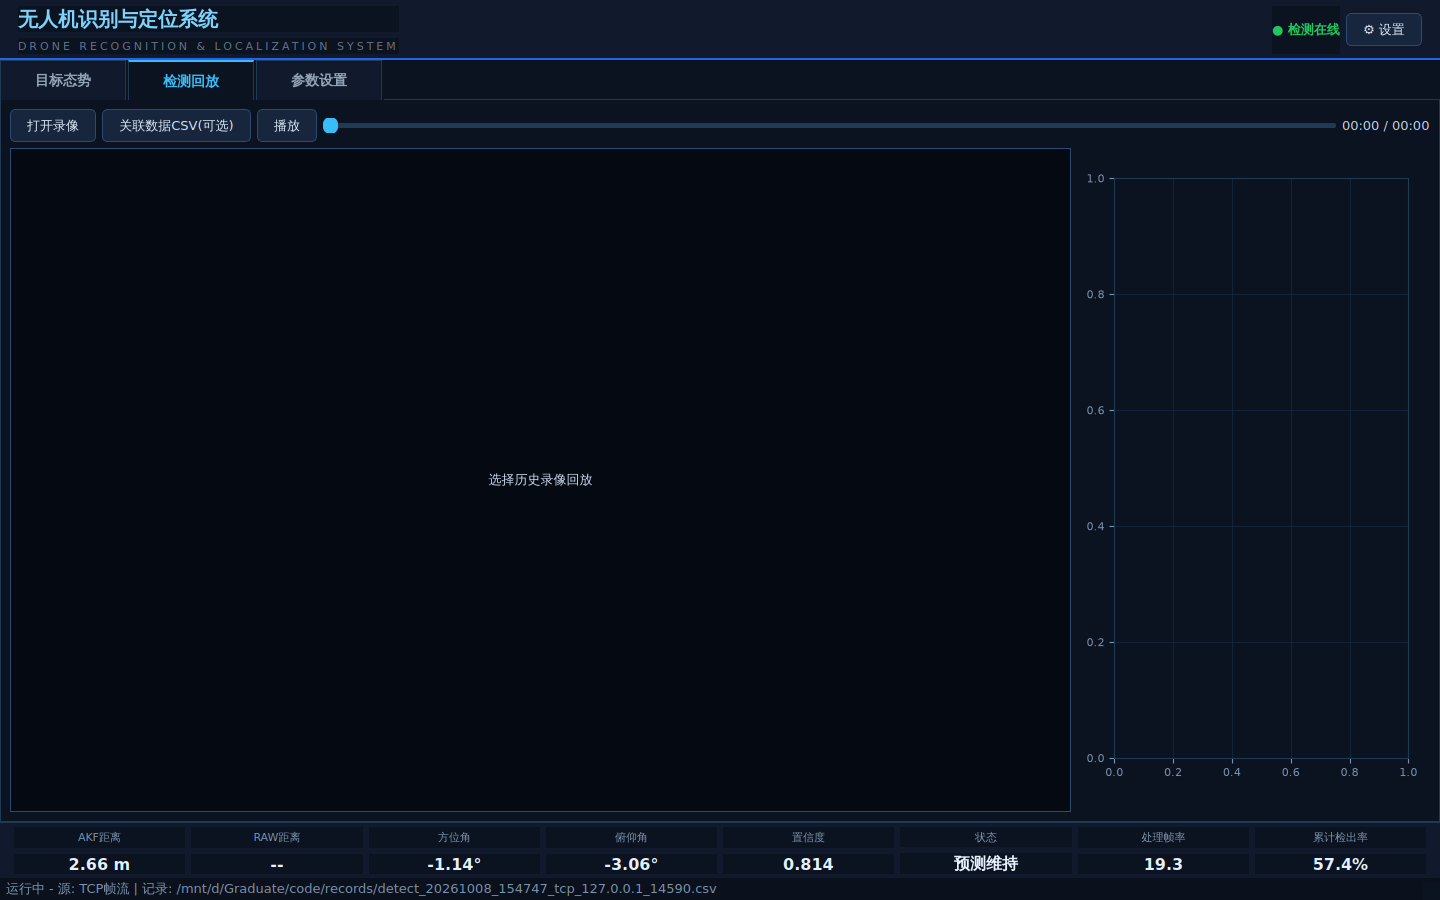
\includegraphics[width=0.85\textwidth]{images/pictures/dashboard_replay.png}
\caption{检测回放页}
\label{fig:dashboard_replay}
\end{figure}

设置页如图~\ref{fig:dashboard_settings} 所示，提供置信度门限、等效尺寸、TCP/UDP 地址、地图锚点、地图模式、是否显示数据面板等参数。修改后点击"保存"，参数写入 JSON 文件，下次启动自动加载。参数的默认值与合法范围在代码中集中定义，避免非法输入导致运行时错误。

\begin{figure}[htbp]
\centering
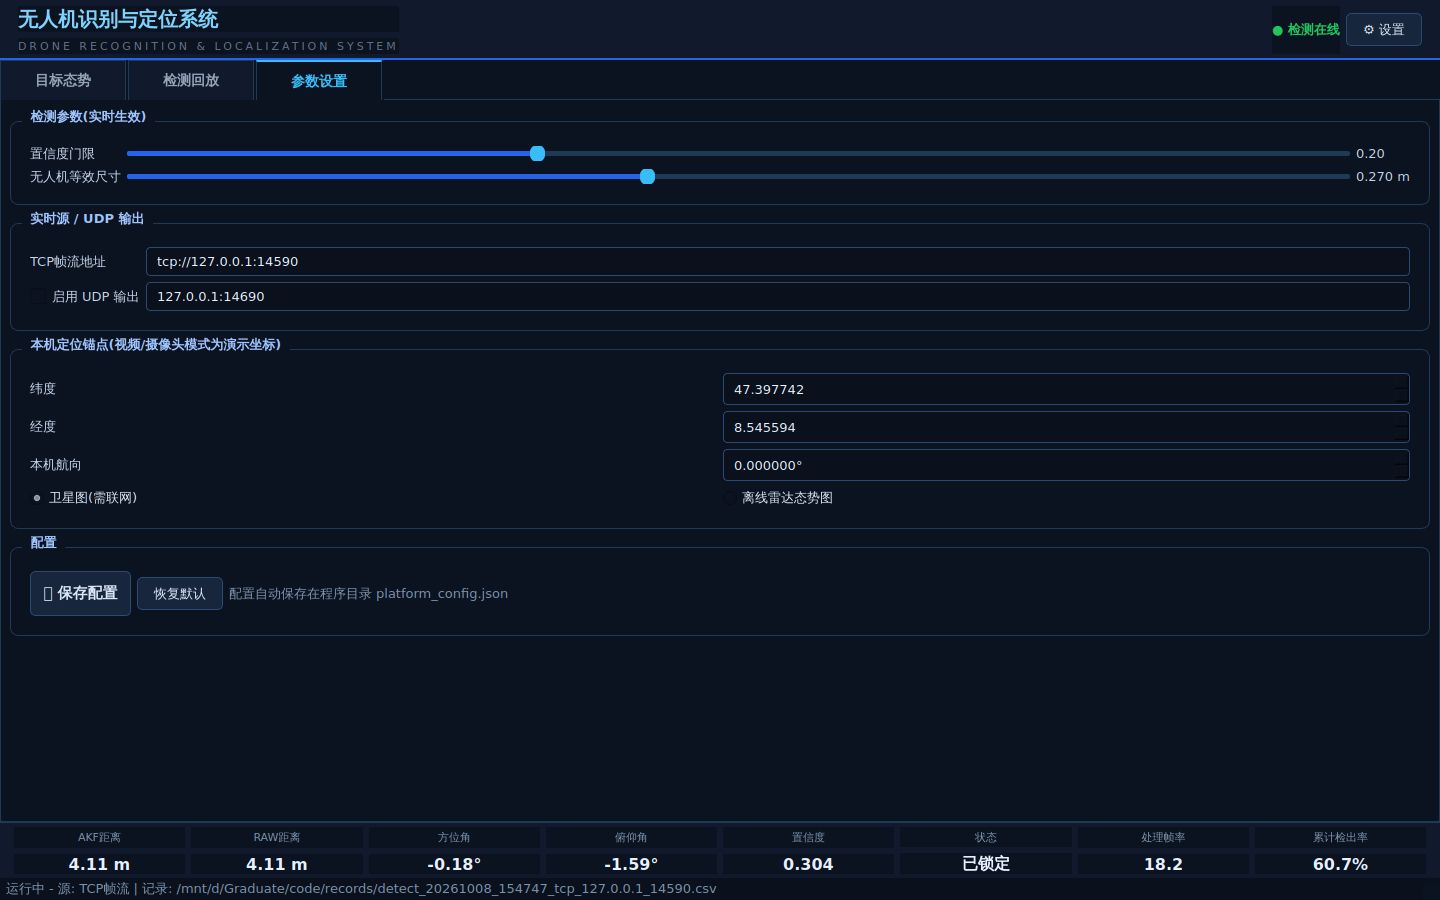
\includegraphics[width=0.85\textwidth]{images/pictures/dashboard_settings.png}
\caption{参数设置页}
\label{fig:dashboard_settings}
\end{figure}

\section{通信协议}

\subsection{视频帧协议}

TCP 帧流协议采用"一行文本头 + 二进制数据"的设计。头部字段依次为序号、时间戳、宽度、高度、字节数，以空格分隔，以换行结束。接收端解析头部后，按字节数读取 JPEG 数据。选择文本头而非二进制头的原因是：便于调试（可直接用 telnet 观察），且字段含义自解释。

\subsection{真值协议}

UDP 真值报文为单行文本，字段以空格分隔，键值对形式。接收端按空格切分，再按等号拆分键值。该协议简单、易于扩展，新增字段不影响旧版接收端。

\subsection{结果协议}

UDP 结果报文为 JSON。选择 JSON 而非自定义二进制的原因是：显示端与上级系统可能使用不同语言，JSON 具有广泛的支持；字段可读，便于联调。报文大小约 300 字节，远小于 UDP 的 1472 字节 MTU，不需要分片。

\section{配置与持久化}

系统配置分为三类：

（1）\textbf{算法参数}：模型路径、输入尺寸、置信度门限、等效尺寸、空域先验、滤波噪声；

（2）\textbf{通信参数}：TCP 地址与端口、真值 UDP 端口、结果 UDP 地址与端口；

（3）\textbf{界面参数}：地图锚点、地图模式、是否显示数据面板、告警阈值。

所有参数保存在一个 JSON 文件中，结构为嵌套字典。程序启动时读取，缺失字段使用默认值填充；保存时保留未知字段，避免版本升级导致配置丢失。这一"宽松读写"策略在实际使用中减少了大量配置兼容问题。

\section{回放与自动化测试}

\subsection{14 用例测试框架}

为系统化验证系统功能，本文设计了 14 个自动化用例，覆盖六类场景：

（1）\textbf{基线检测}（C01--C03）：使用仿真闭环录像，验证检测、跟踪、测距的基本正确性；

（2）\textbf{真实场景}（C04--C05）：使用真实无人机录像，验证跨域能力与远距离边界；

（3）\textbf{门限扫描}（C06--C08）：改变置信度门限，观察锁定率与保持率的变化；

（4）\textbf{尺寸敏感}（C09--C10）：改变等效尺寸，验证测距的线性关系；

（5）\textbf{TCP 遮挡}（C11--C13）：通过实时帧流注入遮挡场景，验证 COAST 机制；

（6）\textbf{摄像头}（C14）：验证 USB 摄像头输入（默认跳过，需要时手动启用）。

每个用例定义输入源、参数、期望指标与判定规则。测试框架按顺序执行用例，收集 CSV，计算锁定率、航迹保持率、首锁时延、置信度均值、距离范围与处理帧率，最后生成汇总表。判定规则为：基线用例要求锁定率不低于 80\%；TCP 遮挡用例要求航迹保持率不低于 70\%；特性刻画用例只统计不判定。

\subsection{测试结果}

测试结果详见第九章。这里强调框架的两个设计要点：其一，\textbf{指标口径统一}：所有用例使用同一套计算函数，避免人工统计的差异；其二，\textbf{失败可复现}：每个用例的输入、参数与随机种子都记录在案，失败时可以单独重跑。

\section{部署与运行维护}

\subsection{运行环境}

系统的开发与测试环境为 Windows 11 + WSL2（Ubuntu 24.04），GPU 为 RTX 4060，Python 3.12，PySide6 6.x，PyTorch 2.x，Ultralytics 8.x，OpenCV 4.x。仿真部分运行在 WSL 中，界面通过 WSLg 显示。

\subsection{启动脚本}

系统提供一键启动脚本，按顺序启动闭环与平台。脚本中固化了以下环境变量：

（1）\texttt{DISPLAY=:0} 与 \texttt{QT\_QPA\_PLATFORM=xcb}：指定 WSLg 显示；

（2）\texttt{QTWEBENGINE\_DISABLE\_SANDBOX=1}：关闭 QtWebEngine 沙箱，避免渲染进程启动失败；

（3）\texttt{QTWEBENGINE\_CHROMIUM\_FLAGS}：启用软渲染与禁用 GPU，解决 WSLg 下地图空白问题。

启动方式必须使用 \texttt{setsid} 而非 \texttt{nohup}。原因是 QtWebEngine 的 zygote 进程需要独立的会话，\texttt{nohup+disown} 方式会导致渲染进程无法启动，表现为地图区域全黑。这一细节在部署文档中已明确记录。

\subsection{常见问题与处理}

表~\ref{tab:deploy_issues} 汇总了部署与运行中的常见问题及处理方法。

\begin{table}[htbp]
\centering
\caption{部署与运行常见问题}
\label{tab:deploy_issues}
\small
\begin{tabularx}{\textwidth}{lX}
\toprule
\textbf{现象} & \textbf{原因与处理} \\
\midrule
地图区域空白 & QtWebEngine 渲染进程未启动；使用 setsid 启动并关闭沙箱 \\
仿真窗口不出画面 & 窗口系统不可用；改用离屏渲染模式 \\
UDP 端口被占用 & 显示端已监听；先停止显示端再启动抓包工具 \\
帧率骤降 & GPU 被其他任务占用，回退到 CPU；检查显卡占用 \\
视频流断开 & 仿真重启或网络抖动；帧源自动重连 \\
内存持续增长 & 帧队列无界；改为有界队列并丢弃旧帧 \\
\bottomrule
\end{tabularx}
\end{table}

\section{本章小结}

本章介绍了系统的需求、架构与实现。系统采用双进程架构，算法端负责检测、跟踪、定位与记录，显示端负责态势、光电、仪表与告警，二者通过 UDP/JSON 通信。算法端以有界队列实现背压控制，保证长时间运行稳定；显示端以 Leaflet 实现卫星地图态势，以自绘控件实现仪表与罗盘；配置以 JSON 持久化，测试以 14 用例自动化框架完成。本章还总结了部署中的典型问题与处理方法，为系统的可复现运行提供了保障。
